%http://www.linux-magazine.com/Online/Blogs/Paw-Prints-Writings-of-the-maddog/Brazil-Free-and-Open-Source-Culture-Is-Economics-Not-Politics
%https://books.google.com.br/books?id=pxAVCgAAQBAJ&pg=PA166&lpg=PA166&dq=Brazil:+Free+and+Open+Source+Culture+Is+Economics,+Not+Politics&source=bl&ots=k5M51pGklX&sig=tCPn4l7OnL7Xzne9cKYowUbYTvo&hl=pt-BR&sa=X&ved=0ahUKEwihkIec0-HPAhUGjpAKHdv6AcwQ6AEIOzAE#v=onepage&q=Brazil%3A%20Free%20and%20Open%20Source%20Culture%20Is%20Economics%2C%20Not%20Politics&f=false
%http://pear.accc.uic.edu/ojs/index.php/fm/article/view/904/813
%https://books.google.com.br/books?id=fEP2smsHVCwC&pg=PA14&lpg=PA14&dq=Brazil:+Free+and+Open+Source+Culture+Is+Economics,+Not+Politics&source=bl&ots=FsxRuW6joV&sig=l_PNwCwjTLl-XBATmeSIVO70Fcs&hl=pt-BR&sa=X&ved=0ahUKEwihkIec0-HPAhUGjpAKHdv6AcwQ6AEISzAG#v=onepage&q=Brazil%3A%20Free%20and%20Open%20Source%20Culture%20Is%20Economics%2C%20Not%20Politics&f=false
\chapter{Projeto da ferramenta}

KDE é conhecido por utilizar as ferramentas e bibliotecas disponibilizadas pela \textit{QT Project}\footnote{Empresa desenvolvedora  de software, famosa pelas suas bibliotecas e \textit{IDEs} de desenvolvimento} na realização do desenvolvimento dos seus projetos. O conhecimento inicial de como utilizar tais ferramentas é de grande valia para o projeto no desenvolvimento da proposta.


\section{Requisitos}

O usuário deve ser capaz de utilizar o plugin para realizar a programa-\\ção de sistemas embarcados, com a ajuda de um \textit{bootloader}, ou utilizando carregadores de código especializado do hardware. Além de ser possível programar, dependendo do caso, o desenvolvedor seria capaz de utilizar o plugin para a realização da depuração do projeto dentro do próprio sistema em desenvolvimento, caso o sistema utilizado por suportar tal comportamento.

A escolha do Arduino como plataforma alvo foi realizada pela sua fácil aquisição, baixo preço e alta popularidade dentre a comunidade civil como um dos microcontroladores mais populares, desta forma, é um bom primeiro passo para a realização da estrutura de software a ser desenvolvida para o plugin.

O sistema deve ter as seguintes funcionalidades para exercer um bom funcionamento para o usuário.
\begin{itemize}
\item O sistema deve permitir ao usuário:
	\subitem A criação de novos projetos e disponibilizar um modelo.
	\subitem Integração de projeto do usuário.
    \subitem Configuração das ferramentas utilizadas.
	\subitem Executar a compilação do projeto.
	\subitem Executar a instalação de ferramentas.
	\subitem Carregar o binário para o sistema embarcado.
\item Os projetos devem ser salvos assim como as configurações.
\item Executar o carregamento utilizando as ferramentas selecionadas.
\item Avisar sobre erros e problemas durante a ocorrência de alguma etapa para o usuário.	
\end{itemize}

Algumas propriedades e restrições do sistema são vitais para seu funcionamento.
\begin{itemize}
\item O sistema deve executar sem acarretar em uma falha durante a execução.
\item A instalação de ferramentas podem ser feitas sem a permissão de administrador.
\item O programa deve executar sem vazamento de memória \cite{Patterson:2008:COD:1502247}.
\item Evitar a manipulação do arquivo por terceiros durante a instalação das dependências.
\end{itemize}

\section{Plataformas suportadas}

Neste projeto, como versão inicial, será suportado as plataformas mais populares da Arduino, validando o suporte para placas com processadores AVR da plataforma, e os sistemas que utilizam \textit{OpenOCD}\footnote{Utilizando majoritariamente em placas com processadores ARM (Arduino DUE, STM32, entre outros).}, resultando num sistema que pode ser utilizado em todas as placas da Arduino\footnote{Com processadores ARM e AVR.}. Outros suportes para sistemas de carregamento podem vir a ser adicionados em futuras versões.


\section{Estrutura do software}

Foi desenvolvido um diagrama de classes (\figref{fig:uml}) que demonstra a proposta de software do plugin. A estrutura do Arduino \textit{toolkit} necessita de certas classes ou funções especiais para sua integração com a proposta do trabalho, além disso, certas classes foram feitas para as interfaces com foco nos usuários menos experientes. Outras camadas têm como proposta uma abstração para as placas de desenvolvimento, lidando com muitas variações de processador e configurações de hardware. 

Esta proposta inicial de UML seria realizada como prova de conceito da integração do KDevelop para sistemas embarcados, desta forma, necessitando de modificações para a criação de classes mais abstratas, permitindo uma melhor incorporação de outras ferramentas de desenvolvimento.o.

\begin{figure}[!htb]
  \centering
  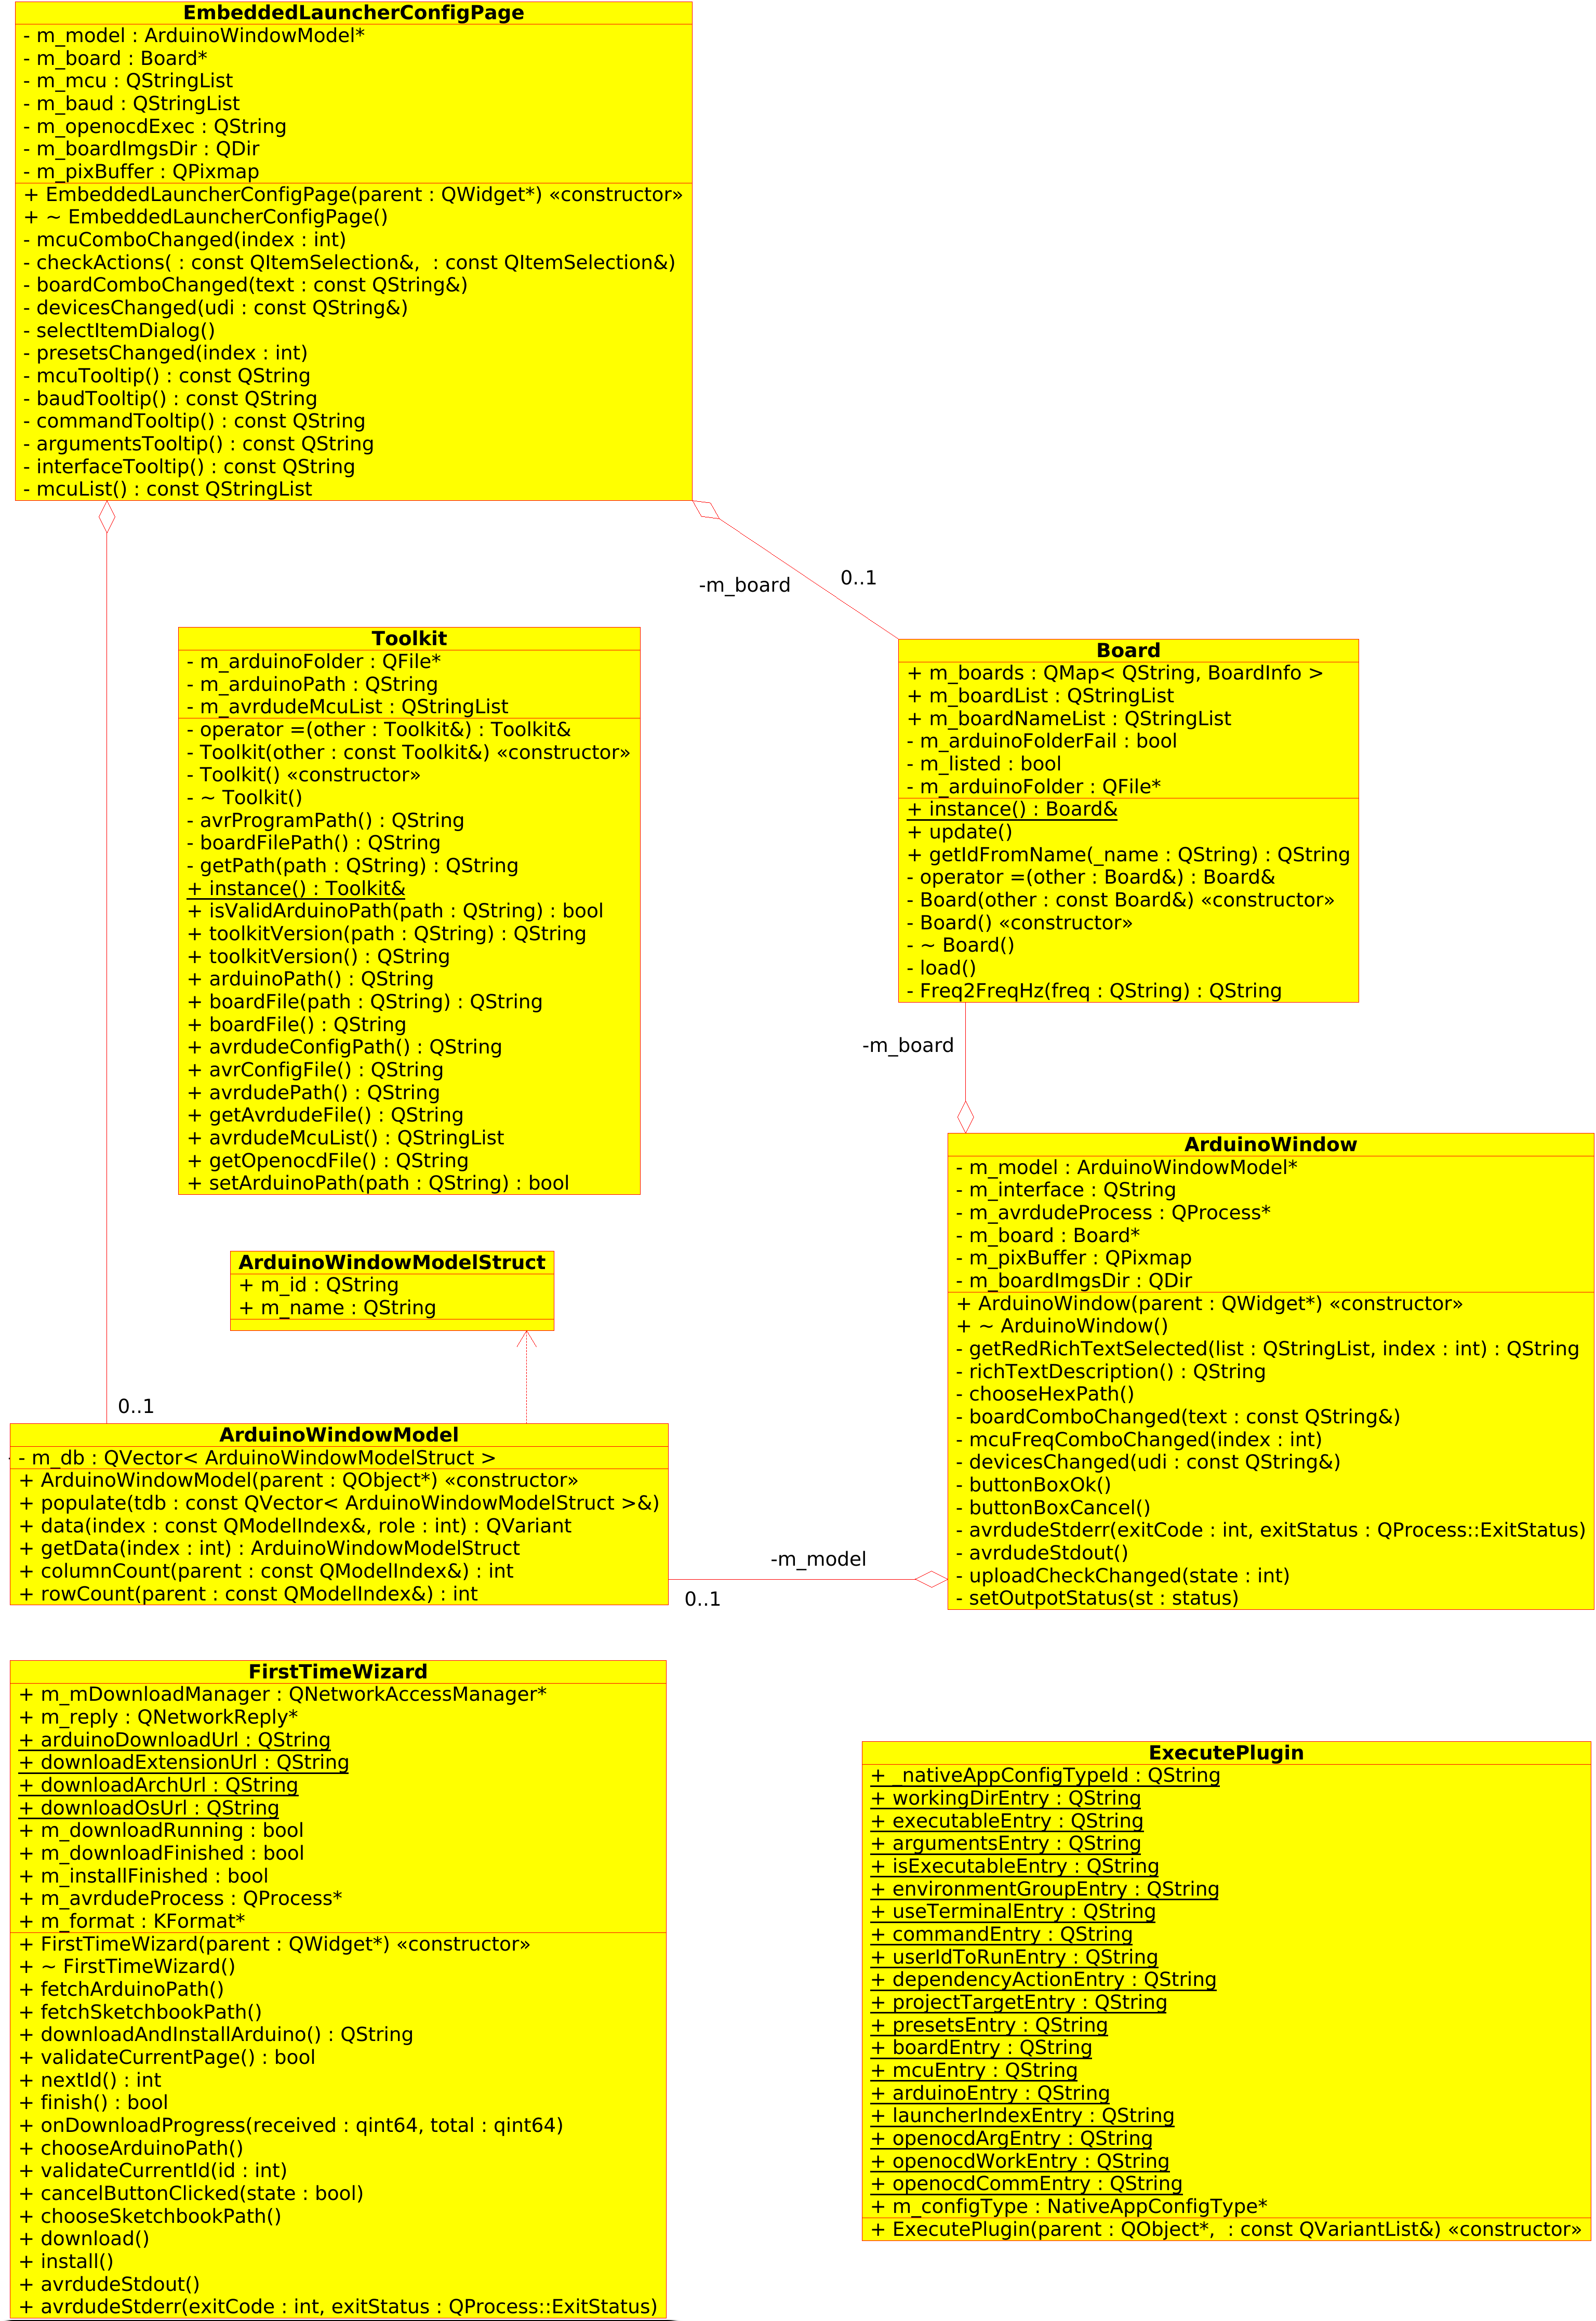
\includegraphics[width=0.85\textwidth]{figuras/uml.png}
  \caption[UML proposto]{Representação do plugin proposto através do diagrama de classes UML.}
  \label{fig:uml}
\end{figure}

\abreviatura{UML}{Unified Modeling Language}


%Em futuras versões mais  ferramentas deverão ser adicionados,
%, serão os primeiros a serem suportados pelo plugin como prova de conceito por apresentarem uma grande quantidade de usuários.
%Como objetivo final do projeto, o usuário deve ser capaz de utilizar o
